\documentclass{beamer}
\mode<presentation>
\usetheme{CambridgeUS}
\usepackage[russian]{babel}
\usepackage[utf8]{inputenc}
\usepackage[T2A]{fontenc}
\usepackage{sansmathaccent}

\usepackage{verbatim}
\usepackage{alltt}

\pdfmapfile{+sansmathaccent.map}
\title[Основы языка Pascal]{Основы языка Pascal}
\author{Наумов Д.А., доц. каф. КТ}
\date[19.09.2019] {Программирование и алгоритмические языки, 2019}

\begin{document}

%ТИТУЛЬНЫЙ СЛАЙД
\begin{frame}
  \titlepage
\end{frame}
  
%СОДЕРЖАНИЕ ЛЕКЦИИ
\begin{frame}
  \frametitle{Содержание лекции}
  \tableofcontents  
\end{frame}

\section{Основные элементы языка}

\begin{frame}{Структура приложения}
\begin{figure}[h]
\centering
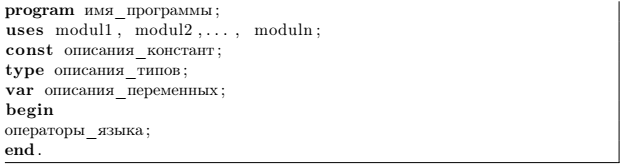
\includegraphics[scale=0.75]{images/lec02-pic01.png}
\end{figure}
\end{frame} 

\begin{frame}{Основные элементы языка}
Алфавит языка:
\begin{figure}[h]
\centering
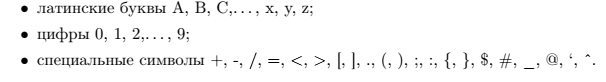
\includegraphics[scale=0.75]{images/lec02-pic02.png}
\end{figure}
Комментарии:
\begin{figure}[h]
\centering
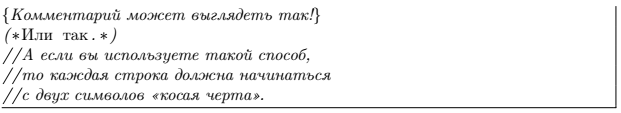
\includegraphics[scale=0.75]{images/lec02-pic03.png}
\end{figure}
\end{frame}

\begin{frame}{Основные элементы языка}
\begin{block}{Идентификатор}
совокупность букв, цифр и символа подчёркивания. 
\end{block}
\begin{itemize}
\item начинается с буквы или символа подчёркивания;
\item используется для именования различных объектов (констант, переменных, меток, типов данных, процедур, функций, модулей, классов) языка;
\item не может содержать пробел;
\item прописные и строчные буквы в именах не различаются;
\item каждое имя (идентификатор) должно быть уникальным и не совпадать
с ключевыми словами.
\end{itemize}
\end{frame}

\begin{frame}{Типы данных}
Данные хранятся в памяти компьютера и могут быть самых различных
типов
\begin{itemize}
\item целые;
\item вещественные числа;
\item символы;
\item строки;
\item массивы...  
\end{itemize}
Тип данных определяет:
\begin{itemize}
\item структуру хранения данных в памяти;
\item область значений, которые могут принимать данные этого типа;
\item множество операций, применимых к данным этого типа. 
\end{itemize}
\end{frame}

\begin{frame}[fragile]
\begin{block}{Переменная}
величина, которая может изменять свое значение.
\end{block}
\begin{itemize}
\item идентификатор (имя) служит для обращения к области памяти, в которой хранится значение;
\item значение переменной можно изменить;
\item перед использованием любая переменная должна быть описана. 
\end{itemize}
Описание переменной:
\begin{alltt}
1  var
2    идентификатор1, идентификатор2,...,идентификаторN: тип;
\end{alltt}
\begin{figure}[h]
\centering
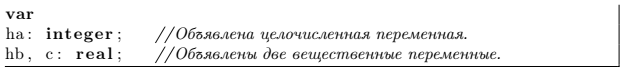
\includegraphics[scale=0.75]{images/lec02-pic04.png}
\end{figure}
\end{frame}

\begin{frame}[fragile]
\begin{block}{Константа}
величина, которая не может изменять свое значение.
\end{block}
Определение константы:
\begin{alltt}
1  var
2    идентификатор = константное_выражение;
\end{alltt}
\begin{figure}[h]
\centering
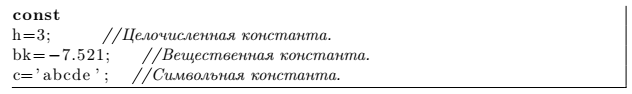
\includegraphics[scale=0.7]{images/lec02-pic05.png}
\end{figure}
\end{frame}

\section{Концепция типов данных}
\subsection{Организация данных в программах}
\begin{frame}[t]
Программирование языке низкого уровня требует точного знания: 
\begin{itemize}
\item как данные представлены в виде последовательности битов;
\item какие машинные команды должны применяться для реализации требуемых операций.
\end{itemize}
Язык высокого уровня обеспечивает следующие возможности:
\begin{itemize}
\item на объекты данных ссылаются с помощью определенных пользователем имен, а не конкретных адресов памяти;
\item объекты данных связаны с типом, определяющим множество значений, которые могут приниматься объектами этого типа, и множество операций, которые могут применяться к объектам этого типа.
\end{itemize}
Хороший механизм типов является ключевым фактором при обеспечении
надежности языка программирования, что имеет первостепенную важность при программировании.
\end{frame} 

\begin{frame}[c]
В общем случае в языке программирования должно быть \emph{множество предопределенных типов данных} и \emph{набор механизмов для спецификации типов}, определяемых пользователем.
\begin{block}{Типы данных}
\begin{enumerate}
\item простые;
	\begin{itemize}
	\item нет внутренней структуры;
	\item могут содержать лишь одно значение;
	\item доступные операции предопределены;	
	\end{itemize}
\item структурные
	\begin{itemize}
	\item состоят из других простых и (или) структурных типов;
	\item могут содержать составные значения;
	\item могут инкапсулировать поведение.	
	\end{itemize}
\end{enumerate}
\end{block}
\end{frame}  

\begin{frame}{Типы данных}
\begin{figure}[h]
\centering
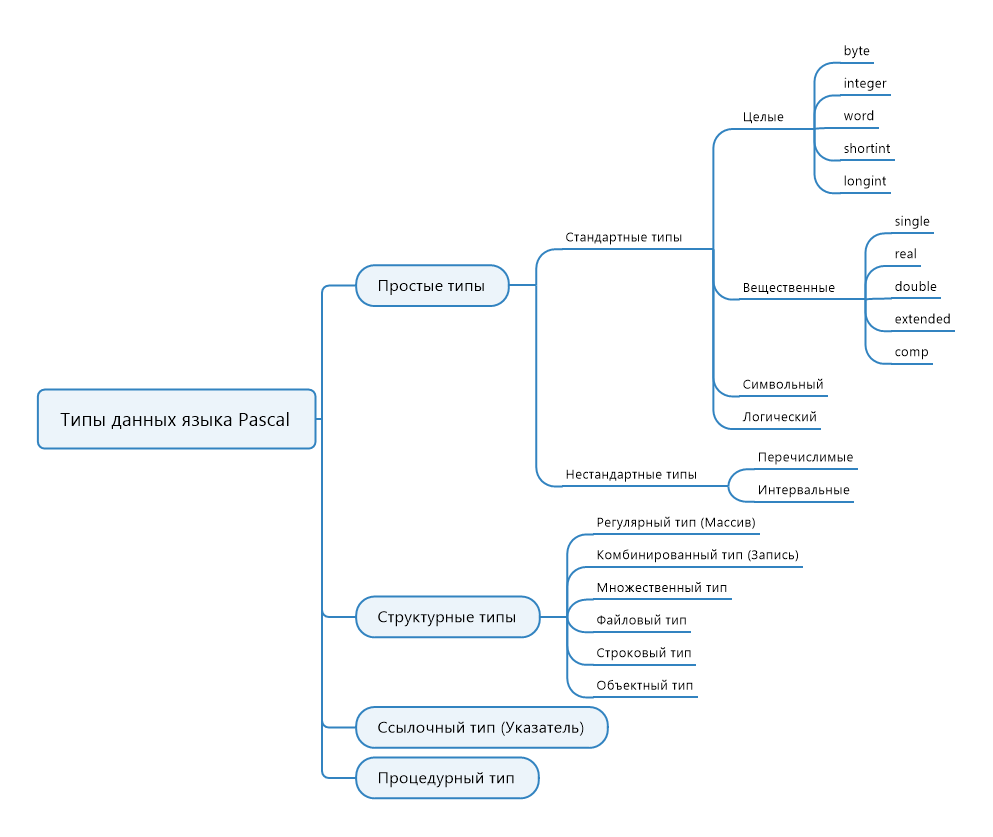
\includegraphics{images/tree_of_types.png}
\end{figure}
\end{frame} 

\begin{frame}
Целочисленные типы данных FreePascal:
\begin{figure}[h]
\centering
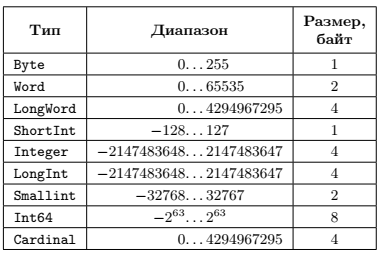
\includegraphics[scale=0.6]{images/lec02-pic06.png}
\end{figure}
Описание целочисленных переменных:
\begin{figure}[h]
\centering
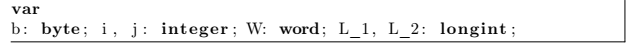
\includegraphics[scale=0.7]{images/lec02-pic07.png}
\end{figure}
\end{frame} 

\begin{frame}
Внутреннее представление вещественного числа:
\begin{figure}[h]
\centering
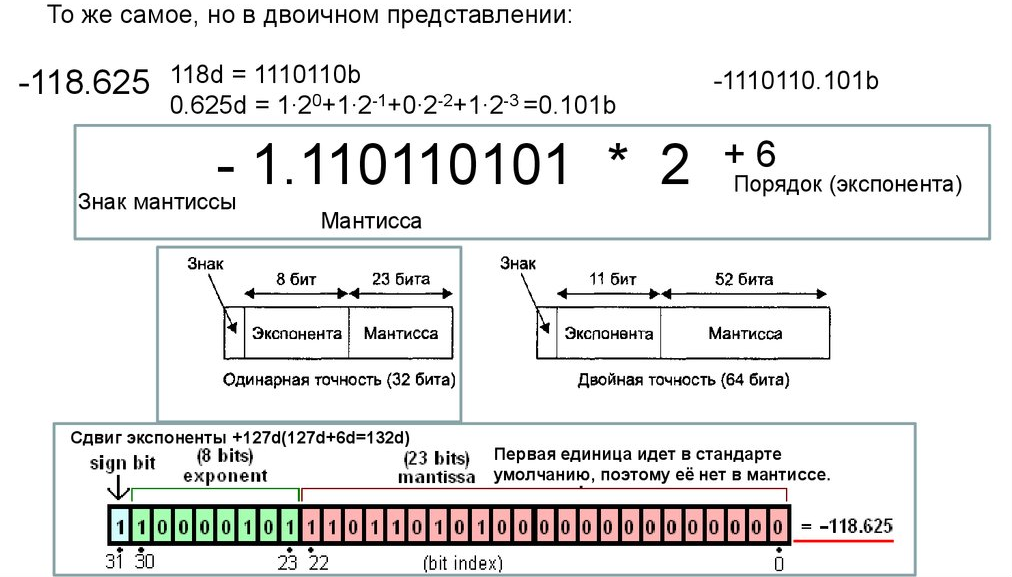
\includegraphics[scale=0.7]{images/lec02-pic09.png}
\end{figure}
\end{frame} 

\begin{frame}
Константы вещественного типа:
\begin{itemize}
\item в формате с фиксированной точкой;
\item в формате с плавающей точкой.
\end{itemize}
Вещественные типы данных FreePascal:
\begin{figure}[h]
\centering
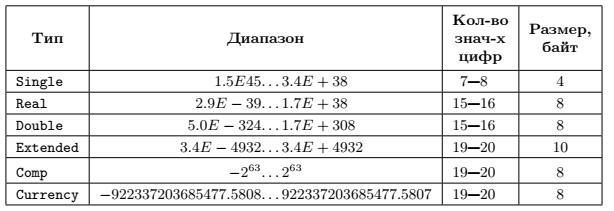
\includegraphics[scale=0.7]{images/lec02-pic08.png}
\end{figure}
\end{frame} 

\begin{frame}{Логический тип данных}
Константы логического типа:
\begin{itemize}
\item True - логическая истина;
\item False - логическая ложь.
\end{itemize}
Логические типы данных FreePascal:
\begin{figure}[h]
\centering
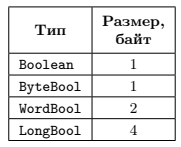
\includegraphics[scale=0.75]{images/lec02-pic10.png}
\end{figure}
\end{frame} 

\begin{frame}[fragile]
\textbf{Перечисляемый тип} данных относится к нестандартным порядковым типам и определяется набором идентификаторов, с которыми могут совпадать значения переменных этого типа.
\begin{alltt}
1  type TDay = (MO, TU, WE, TH, FR, SA, SU);
2  var  D: TDay; 	
3  (* ORD (WE) = 2 *)
\end{alltt}
Максимальная мощность перечисляемого типа - 256 значений.
\begin{alltt}
(* типы эквивалентны по внутреннему представлению...*)
1  type TColors = (black, red, white );
2       TOrdenal=(one, two, three);
3       TDays=(monday, thesday, wednesday); 	
4  var  col: TColor; num: TOrdenal; day: TDays;
(* допустимые операторы присваивания *)
5  col := black; num := two; day := monday;
(* недопустимые операторы присваивания *)
6  col := two; day := black;
\end{alltt}
\end{frame}
   
\begin{frame}[fragile]
Для перечисляемых типов определены стандартные функции PRED, SUCC и ORD, имеющие тот же смысл, что и для стандартных скалярных типов.
\begin{alltt}
1  type TColors = (black, red, white);
2  (* SUCC(red) = white *)
3  (* PRED(red) = black *)
4  (* ORD(red) = 1 *)
\end{alltt}
\begin{itemize}
\item значения перечисляемого типа должны быть определены только идентификатором (именем);
\item нельзя присваивать переменной значение из описания другого типа;
\item недопустимо описание двух и более перечисляемых типов с совпадающими значениями;
\item нельзя значения перечисляемого типа использовать для ввода и вывода.
\end{itemize}
\begin{alltt}
1 type TColor1 = (red, yellow, blue);
2      TColor2 = (green, blue, gray);
\end{alltt}
\end{frame}   

\begin{frame}[fragile]
\textbf{Ограниченный тип данных} относится к нестандартным порядковыми
типам, образуется на основе порядковых типов, называемых базовыми,
путём ограничения диапазона значений этих типов заданием минимального и максимального значений.
\begin{alltt}
1  type TDay = (MO, TU, WE, TH, FR, SA, SU);
2       TNumber = 10..25;
3       TChars = 'c'..'x';
4       TWeekDays = SA..SU;
\end{alltt}
\begin{itemize}
\item базовым типом для создания ограниченного типа может быть любой
порядковый тип;
\item два символа ".." рассматриваются как один символ, поэтому между
ними не допустимы пробелы;
\item необходимо, чтобы левая граница диапазона не превышала его правую
границу.
\end{itemize}
\end{frame}
   
\subsection{Слабая и сильная типизация}
\begin{frame}[fragile]
\begin{block}{Особенности слабой типизации}
\begin{itemize}
\item операция, которая может восприниматься машиной как корректная,
может быть некорректной на абстрактном уровне программы;
\begin{alltt}
1  var c: char;
2  c := 10;
\end{alltt}
\item для сохранения корректности предусмотрено выполнение операции преобразования типа;
\begin{alltt}
1  var x,y: real; 
2  var i,j,k: integer; 
3  i := x;
4  k := y - j;
\end{alltt}
\item увеличение гибкости, обеспечиваемое слабой типизацией, является слишком дорогой ценой за резкое уменьшение ясности программ и необходимость дополнительного контроля во время работы компилятора.	
\end{itemize}
\end{block}
\end{frame}   

\begin{frame}[fragile]
\begin{block}{Особенности сильной типизации}
\begin{itemize}
\item каждый объект обладает уникальным типом;
\item тип определяет множество значений и множество операций;
\item тип присваиваемого значения и тип объекта данных, которому производится присваивание, должны быть эквивалентны;
\item применяемая к объекту операция должна принадлежать множеству операций, определяемому типом объекта.
\end{itemize}
\begin{alltt}
1  var x: real;
2      i: integer;
3      b: boolean;
4      c: char;
5  i := 'A' (*разные типы в левой и правой частях*)
6  x := i;
7  i := i or 10; (*недопустимая операция*)
\end{alltt}
\end{block}
\end{frame}   

\begin{frame}[fragile]
Преимущество сильной типизации: программисту разрешается определять при описании типа свои собственные типы. 

\begin{alltt}
1  type 
2    TAge = 0..200;
3    TIndex = 1..10;
4  var 
5    age, total_age : TAge;
2    i: TIndex;
3  begin
4    total_age := 0;
4    for i := 1 to 10 do begin
5      readln(age);
6      total_age := total_age + age;
7    end;
8    writeln(total_age);
9  end.
\end{alltt}
\end{frame}
   
\begin{frame}[fragile]
Имеются две различные основы для вычисления эквивалентности типов данных:
\begin{itemize}
\item структурная эквивалентность: два объекта принадлежат эквивалентным типам, если у них одинаковая структура;
\item именная эквивалентность: два объекта принадлежат эквивалентным типам, если они описаны с помощью одного и того же типа.
\end{itemize}

В языке Pascal принят принцип именной эквивалентности типов, устанавливающий, что два типа T1 и T2 эквивалентны, если выполняется одно из следующих условий:
\begin{itemize}
\item T1 и T2 — одно и то же имя типа;
\item Тип T2 описан с использованием типа T1 равенством вида type T2=T1; или последовательностью подобного вида равенств.
\end{itemize}
\begin{alltt}
1  type T1 = integer;
2    T3 = T1;
3    T2 = T3;
4    T4 = 1..10;
5    T5 = 1..10; 	
\end{alltt}
\end{frame}   

\begin{frame}
\begin{block}{Выражение}
задаёт порядок выполнения действий над данными и состоит из операндов (констант, переменных, обращений к функциям), круглых скобок и знаков операций.
\end{block}
\begin{block}{Операнд}
это аргумент операции.
\end{block}
Каждая операция:
\begin{itemize}
\item имеет знак операции;
\item определяет количество операндов;
\item определяет допустимый тип операндов;
\item имеет приоритет;
\item имеет ассоциативность.
\end{itemize}
\end{frame}

\begin{frame}{Операции}
\begin{figure}[h]
\centering
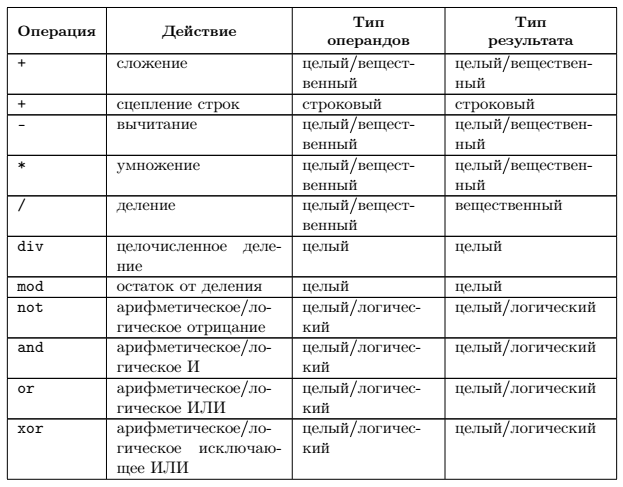
\includegraphics[scale=0.75]{images/lec02-pic11.png}
\end{figure}
\end{frame} 

\begin{frame}{Операции}
\begin{figure}[h]
\centering
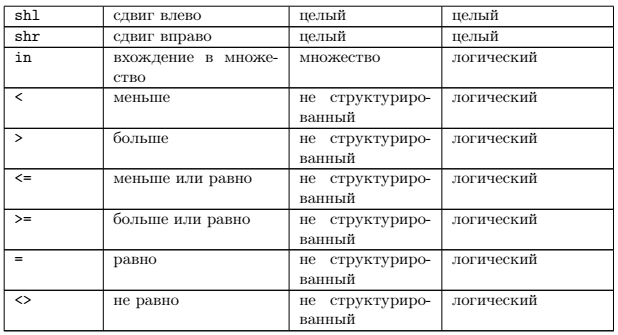
\includegraphics[scale=0.75]{images/lec02-pic12.png}
\end{figure}
\end{frame} 

\begin{frame}{Стандартные функции}
\begin{figure}[h]
\centering
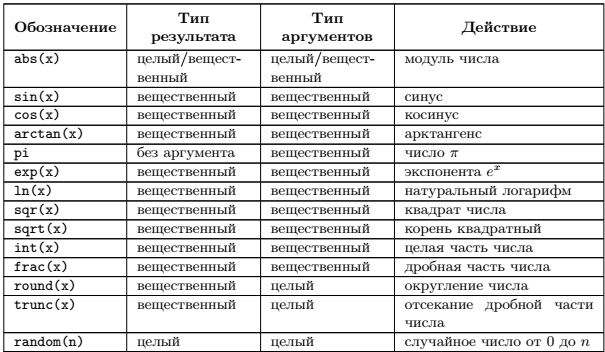
\includegraphics[scale=0.75]{images/lec02-pic13.png}
\end{figure}
\end{frame} 

\begin{frame}
\begin{block}{Оператор (команда, инструкция)}
наименьшая автономная часть языка программирования.
\end{block}
\begin{itemize}
\item оператор присваивания;
\item операторы ввода-вывода;
\item составной оператор;
\item условные операторы;
\item циклические операторы;
\item оператор вызова процедуры.
\end{itemize}
\end{frame}

\begin{frame}[fragile]
Синтаксическая форма оператора присваивания:
\begin{alltt}
1  L-выражение := R-выражение;
\end{alltt}
\begin{itemize}
\item L-выражение в результате вычисления должно указывать на переменную;
\item R-выражение в результате вычисления должно быть совместимым по присваиванию с L-выражением;
\end{itemize}
Этапы выполнения оператора присваивания:
\begin{enumerate}
\item вычисляется значение R-выражение (в соотвествии с приоритетом операций);
\item вычисляется L-выражение;
\item значение R-выражения приводится к типу L-выражения;
\item в ячейку памяти (вычисленное на шаге 2) записывается вычисленное на шаге 3 значение.
\end{enumerate}
\end{frame}

\begin{frame}[fragile]
Операторы вывода:
\begin{alltt}
1  Write(Выр1:Фрмт1, Выр2:Фрмт2,...);
2  Writeln(Выр1:Фрмт1, Выр2:Фрмт2,...);
\end{alltt}
\begin{itemize}
\item Выр1, Выр2,... - выражения, которые будут выведены;
\item Фрмт1, Фрмт2,...  - формат вывода может задавать ширину поля (выражение целого типа) для вывода значений выражения и количество разрядов (выражение целого типа) для вывода выражения вещественного типа в формате с фиксированной точкой.
\end{itemize}
Операторы ввода:
\begin{alltt}
1  Read(Выражение1, Выражение2, ...);
2  Readln(Выражение1, Выражение2, ...);
\end{alltt}
\end{frame}

\end{document}
